We illustrate and compare Bayesian and frequentist view points on GP with a simple example (Fig. \ref{fig:BayesVSFreq}). We show how in a simple model, two outliers can bias a maximum a posteriori inference. The data where generated with:
\begin{equation}
\label{eq:line1}
y = 2x + 15
\end{equation}
and outliers are generated with a parallel line:
\begin{equation}
\label{eq:line2}
\hat{y} = 2x + 40.
\end{equation}
We add some small amount of white noise. We generate eight data points with (\ref{eq:line1}) and two with (\ref{eq:line2}). Since we suspect the underlying data generating mechanism to be linear, we fit a linear kernel with a constant covariance as intercept and some white noise.
\begin{equation}
\mathbf{K} = \text{LIN} + \text{C} + \text{WN}
\end{equation}
where we the upper case matrix notation denotes the covariance matrix of the complete training data. Omitting the scaling parameter for the linear kernel, there are two hyperparameters to learn, that is the noise variance and the hyper-parameter for the constant function. Maximum a posteriori inference fits the single one best line and accounts for the outliers with a large noise scaling parameter. MH does better. It assigns a small amount of probability mass to a different scaling parameter and a larger constant. The resulting prediction (indicating with the predictive mean in figure \ref{fig:BayesVSFreq}) is closer to the true underlying function.   

\begin{figure}
        \centering
        \begin{subfigure}[b]{0.49\textwidth} \centering
              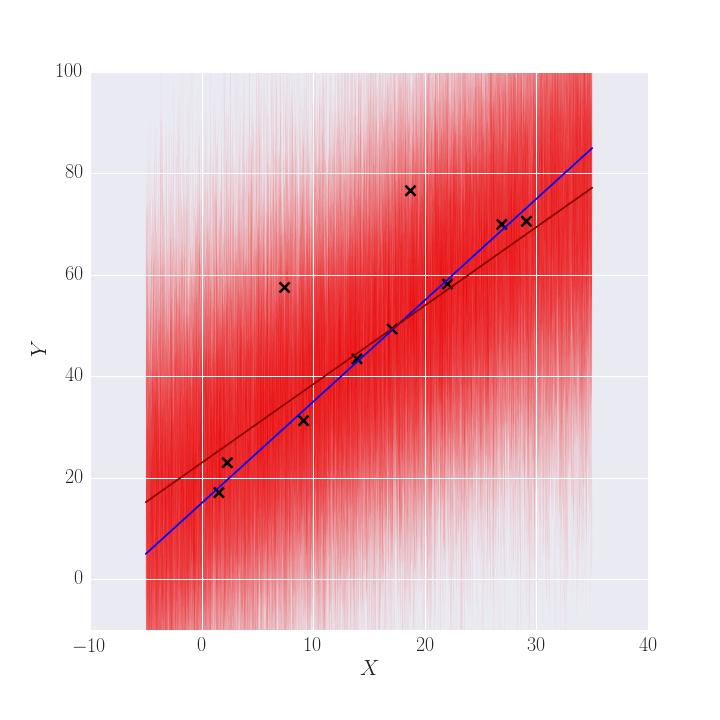
\includegraphics[height=7.5cm]{figs/MAP_linear.png}
              \caption{MAP}
                \label{fig:maplin}
        \end{subfigure}%
        \begin{subfigure}[b]{0.49\textwidth} \centering
            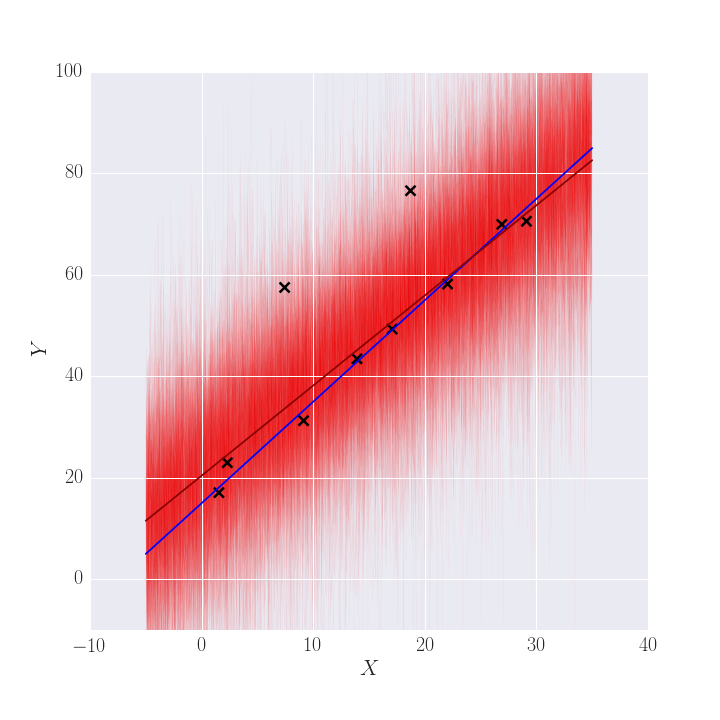
\includegraphics[height=7.5cm]{figs/MH_linear.png}
            \caption{MH}
                \label{fig:mhlin}
        \end{subfigure}%
        \caption{(a) depicts MAP inference on the data, (b) depicts MH for hyperparameter inference. The blue line is the actual data generating function. Red are samples drawn from the posterior. The dark red line is the posterior predictive mean. We see that the MH shifts the posterior closer to the ground truth than MAP.  }\label{fig:BayesVSFreq}
\end{figure}

